\documentclass[12pt,a4paper]{report}
\usepackage[utf8]{inputenc}
\usepackage[T1]{fontenc}
\usepackage{graphicx}
\usepackage{geometry}
\usepackage{setspace}
\usepackage{titlesec}
\usepackage{microtype}
\usepackage{xurl}
\usepackage{hyperref}
\usepackage{amsmath}
\usepackage{array}
\usepackage{booktabs}
\usepackage{longtable}
\usepackage{tabularx}
\usepackage{enumitem}
\usepackage{tikz}
\usetikzlibrary{arrows.meta,positioning,shapes.geometric,fit,calc}
\geometry{a4paper, margin=1in}
\hypersetup{colorlinks=true,linkcolor=black,citecolor=black,urlcolor=blue,pageanchor=false}
\setlength{\parindent}{1.25cm}
\setlength{\parskip}{0pt}
\setlist{nosep,leftmargin=*}
\newcommand{\projectname}{FedLedger}
\newcommand{\reporttitle}{Privacy Preserving Federated Learning for Multi-Institutional Pneumonia Prediction Using Blockchain}
\newcolumntype{Y}{>{\raggedright\arraybackslash}X}
\setlength{\emergencystretch}{2em}
% Supply the institution-approved logo beside this .tex file when available.
\newcommand{\institutionlogo}[1]{%
  \IfFileExists{MITS_LOGO.pdf}{\includegraphics[width=#1]{MITS_LOGO.pdf}}{%
    \fbox{\parbox[c][1.8cm][c]{#1}{\centering Institution logo\\(supply MITS\_LOGO.pdf)}}}}
% Institutional names, signatures, degree wording and dates require departmental confirmation.
% The original names are retained; conflicting coordinator names need author review.

\begin{document}

% Front page
\begin{titlepage}
    \begin{center}
        \institutionlogo{0.38\textwidth} \\
        \vspace{1cm}
        {\parbox{0.9\textwidth}{\centering\LARGE\textbf{\reporttitle}}} \\
        \vspace{1cm}
        \large
        Project Report submitted in partial fulfillment for the degree \\
        of \\
        \textbf{B.Tech in Computer Science and Engineering} \\
        \vspace{0.5cm}
        Submitted by \\
        \textbf{JAIS MATHEW (Reg No: MUT23CS079)} \\
        \textbf{SHAUN BINOY (Reg No: MUT23CS136)} \\
        \textbf{R AJIT (Reg No: MUT23CS128)} \\
        \textbf{VIVEK SASHIDHARAN (Reg No: MUT23CS148)} \\
        \vspace{1cm}
        \Large
        \textbf{Muthoot Institute of Technology and Science Kochi (Autonomous)} \\
        \vspace{0.5cm}
        \textbf{Department of Computer Science and Engineering} \\
        (Affiliated to APJ Abdul Kalam Technological University) \\
        \vspace{0.5cm}
        \textbf{OCTOBER 2026}
    \end{center}
\end{titlepage}
\hypersetup{pageanchor=true}

\pagenumbering{roman}

% Certificate
\chapter*{Certificate}
\addcontentsline{toc}{chapter}{Certificate}
\begin{center}
    \institutionlogo{0.32\textwidth} \\
    \vspace{0.5cm}
    \textbf{DEPARTMENT OF COMPUTER SCIENCE AND ENGINEERING} \\
    \vspace{1cm}
    {\Large\textbf{CERTIFICATE}}
\end{center}
\vspace{0.8cm}
This is to certify that the Project Phase I report entitled \textbf{``\reporttitle''}, submitted by the students named on the title page of Semester VII, is a bonafide account of the work carried out by them under our supervision during the academic year 2026--27.

\vspace{2.4cm}
\begin{center}
\begin{tabular}{p{0.29\textwidth} p{0.29\textwidth} p{0.34\textwidth}}
\textbf{Guide} & \textbf{Coordinator} & \textbf{Head of the Department} \\
Ms. Mithu Mary George & Dr. Saira Varghese & Dr. Anishin Raj M M \\
Asst. Professor & Assoc. Professor & Professor \\
Dept. of CSE & Dept. of CSE & Dept. of CSE
\end{tabular}
\end{center}

\newpage
% Declaration
\chapter*{Declaration}
\addcontentsline{toc}{chapter}{Declaration}
We hereby declare that this submission is our own work and that, to the best of our knowledge and belief, it contains no material previously written by another person nor material which has been accepted for the award of any other degree or diploma of the university or other institute of higher learning, except where due acknowledgement has been made in the text.

The verified Turnitin similarity percentage and the corresponding report must be inserted after the institutional similarity check is completed. No percentage is stated here because a verified result was not included in the supplied project context.

\vspace{1.2cm}
\noindent JAIS MATHEW (Reg No: MUT23CS079) \\
SHAUN BINOY (Reg No: MUT23CS136) \\
R AJIT (Reg No: MUT23CS128) \\
VIVEK SASHIDHARAN (Reg No: MUT23CS148) \\
\vspace{1cm}
\noindent Place: Kochi \\
Date: [insert actual submission date]

\newpage
% Acknowledgements
\chapter*{Acknowledgements}
\addcontentsline{toc}{chapter}{Acknowledgements}
We express our sincere gratitude to the management of Muthoot Institute of Technology and Science for providing the facilities and academic environment required to undertake this project. We thank Dr. Neelakantan P. C., Principal, Muthoot Institute of Technology and Science, and Dr. Anishin Raj M M, Head of the Department of Computer Science and Engineering, for their support.

We are grateful to our project guide, Ms. Mithu Mary George, for guidance, feedback, and encouragement throughout the project. We also thank the project coordinators, Dr. Indu M T and Ms. Neethu Krishna, for their valuable reviews and suggestions. Finally, we thank everyone who contributed directly or indirectly to the completion of this work.

\newpage
% Abstract
\chapter*{Abstract}
\addcontentsline{toc}{chapter}{Abstract}
Medical image data are distributed across institutions and are subject to privacy and governance constraints that can limit centralized model development. FedLedger is a local research prototype for studying a federated workflow for binary chest-radiograph classification into NORMAL and PNEUMONIA. Each simulated hospital trains a ResNet-18 model on its own image partition using FedProx, while a coordinator receives model artifacts and peer-validation evidence. The prototype adds a project-specific acceptance gate and validation-aware aggregation; these are extensions implemented by this project and are not properties of FedProx itself. Model checkpoints and validation reports are exchanged through a local IPFS service, and a local Ethereum-compatible development chain records participant authorization, artifact references, and validation commitments. A browser-based administrator and hospital portal is supported by a Python HTTP service and SQLite coordination store.

The saved project evidence includes an earlier architecture experiment and multiple later portal campaigns. An earlier twenty-round architecture experiment selected round 11 using validation balanced accuracy. Later one-round dashboard campaigns completed the end-to-end workflow with three simulated hospitals. One documented smoke campaign reported pooled validation accuracy of 98.3013\%, but subsequent image review identified a probable transformed-image family crossing that campaign's training/validation boundary. These values are therefore preliminary workflow evidence, not independent test performance or evidence of clinical validity. A reviewed staging copy exists, but the inspected evidence does not establish a completed evaluation of that corrected version. This report describes the architecture, related work, implementation, experiment boundaries, and next steps toward a patient-wise independent evaluation.

\noindent\textbf{Keywords:} federated learning, FedProx, blockchain, IPFS, pneumonia classification, chest radiograph, peer validation

\newpage
\tableofcontents
\newpage
\addcontentsline{toc}{chapter}{List of Figures}
\listoffigures
\newpage
\addcontentsline{toc}{chapter}{List of Tables}
\listoftables
\newpage
\chapter*{Abbreviations}
\addcontentsline{toc}{chapter}{Abbreviations}
\begin{tabularx}{\textwidth}{>{\bfseries}p{0.20\textwidth}Y}
API & Application Programming Interface \\
BA & Balanced Accuracy \\
CID & Content Identifier \\
FL & Federated Learning \\
FedProx & Federated Proximal Optimization \\
IPFS & InterPlanetary File System \\
IID & Independent and Identically Distributed \\
ML & Machine Learning \\
P2P & Peer-to-Peer \\
ROC-AUC & Area Under the Receiver Operating Characteristic Curve \\
\end{tabularx}

\newpage
\pagenumbering{arabic}
\def\theHpage{arabic.\arabic{page}}
\doublespacing

% Chapter 1
\chapter{Introduction}
\section{Background}
Deep learning can learn visual patterns from medical images, but training data are commonly held by separate institutions. Directly pooling those images can be constrained by privacy, governance, and operational requirements. Federated learning (FL) offers a collaborative alternative: participating sites train local models and contribute model updates while retaining their source images. FL reduces the need to transfer raw images, but it does not by itself guarantee that updates cannot leak information, that a participant is honest, or that a model generalizes to new patients.

Blockchain-based FL research uses a distributed ledger to record coordination and model-update commitments. Reviews identify potential benefits in auditability and trust management while also noting trade-offs in throughput, storage, privacy, and deployment complexity \cite{wang2026bcfl,zhu2023blockfed}. FedLedger combines local hospital-style model training with peer assessment, content-addressed artifact storage, and ledger records. The system is a research prototype operated on local development services; its hospitals and data partitions are simulated.

\section{Problem Statement}
Developing a shared pneumonia image classifier from data held by separate hospitals presents two related problems. First, a central data pool is undesirable for the intended privacy-preserving workflow, while local datasets may have different sizes and class proportions. Second, a conventional coordinator's model selection and update handling need explicit provenance and review evidence if participants are to inspect how a global version was formed. The project therefore investigates a controlled prototype that leaves source images in local partitions, records model artifact references and validation commitments, and applies a pre-defined peer acceptance rule before aggregation.

The work does not establish a clinically validated diagnostic tool. It does not implement formal differential privacy or secure aggregation, and blockchain records do not prove that data labels, peer evaluations, or predictions are medically correct.

\section{Objectives}
\begin{enumerate}
    \item Build an end-to-end prototype for simulated multi-hospital training of a two-class chest-radiograph classifier.
    \item Train a ResNet-18 using local data and the FedProx objective to reduce local drift from the incoming global model.
    \item Evaluate peer-submitted models against each reviewer's local validation data and apply a documented update gate.
    \item Combine accepted updates with sample-count and peer-validation-aware weights, or retain the incoming model when all updates are rejected.
    \item Store checkpoint and report artifacts in IPFS and record authorization, content references, and validation commitments on a local development blockchain.
    \item Provide administrator and hospital interfaces for enrollment, campaign participation, progress review, and audit.
    \item Report preliminary validation evidence separately from independent test evaluation and identify the work required for a defensible follow-up study.
\end{enumerate}

\section{Scope and Contributions}
The prototype covers local data registration, simulated hospital enrollment, campaign configuration, round coordination, model training and review, gated aggregation, artifact storage, blockchain references, dashboards, and model-version prediction for research use. A campaign freezes participant and data references before training. The registered configuration uses exactly three hospitals, three local epochs, FedProx $\mu=0.01$, and seed 42. Campaigns declare a round count within the approved maximum; completed one-round smoke campaigns must not be described as twenty-round campaigns.

The project contribution is an integrated implementation and experiment workflow, not a new FL optimizer or a claim of clinical performance. In particular, the peer gate and validation-aware aggregation are project-specific decision rules layered around FedProx. No current FedAvg comparison result is established, and the smoke results are not an independent held-out test.

% Chapter 2
\chapter{Literature Review}
\section{Introduction}
The reviewed papers cover three themes: blockchain-enabled coordination and security for FL; privacy-preserving and robust update handling; and federated medical-image learning under institutional heterogeneity. The two designated base papers provide broad surveys, while eight additional studies provide system designs or medical-learning evaluations. Foundational ResNet and FedProx references are also included. Together, they motivate the architecture but do not validate the performance or security claims of this project.

\section{Related Work}
\subsection{Base Paper 1: Blockchain-Secured Federated Learning in Medicine}
In the 2026 Journal of Medical Internet Research article, Wang et al. present a systematic review of blockchain-based federated learning (BCFL) in the medical field \cite{wang2026bcfl}. The review synthesizes medical blockchain--FL research and discusses medical data sharing, connected medical devices, public-health applications, and telemedicine. The review categorizes integration patterns and discusses how a ledger can support traceability and coordination alongside FL. It also emphasizes unresolved practical issues, including interoperability, compute and communication overhead, privacy concerns, limited external validation, and the gap between simulated systems and clinical deployments. This paper is relevant to the prototype's audit-focused design, while its synthesis cautions against equating a local proof of workflow with deployment readiness.

\subsection{Base Paper 2: Blockchain-Empowered Federated Learning Survey}
In their 2023 ACM Computing Surveys article, Zhu et al. organize blockchain-empowered FL into decoupled, coupled, and overlapped system models, and survey challenges involving coordination, aggregation, client selection, incentives, and security \cite{zhu2023blockfed}. The taxonomy is useful for describing the boundary between the project's off-chain training and aggregation and its on-chain authorization and commitment records. As a survey, it maps solution families rather than establishing that any one architecture is optimal for a particular medical task; system choices still require workload-specific evaluation.

\subsection{Biscotti: A Blockchain System for Private and Secure Federated Learning}
In their 2021 IEEE Transactions on Parallel and Distributed Systems paper, Shayan et al. propose Biscotti, a decentralized peer-to-peer system that combines blockchain and cryptographic mechanisms to coordinate collaborative learning without relying on a single trusted coordinator \cite{shayan2021biscotti}. Their evaluation reports privacy and performance protection in a setting with up to 30\% adversarial clients; the paper also addresses fault tolerance and system scale. This work demonstrates a richer adversarial and privacy design space than the present prototype. FedLedger retains a coordinator and does not implement Biscotti's cryptographic privacy protocol; it therefore must not be described as decentralized or Byzantine-robust in the same sense.

\subsection{Blockchain FL with Committee Consensus}
In their 2021 IEEE Network paper, Li et al. introduce BFLC, a blockchain-based decentralized FL framework in which committee consensus is used to reduce consensus computation and mitigate malicious participation \cite{li2021bflc}. Their evaluation uses FISCO with PBFT consensus, AlexNet, and the FEMNIST handwritten-character dataset, comparing BFLC with basic FL and stand-alone training. The paper informs the use of blockchain for model-update coordination, but its committee consensus and dataset differ from this project's local Hardhat chain and chest-radiograph workflow. A local development chain is not evidence of equivalent consensus, scalability, or resilience.

\subsection{Decentralized Coordination for Resilient FL}
In their 2025 Computer Communications article, Ferretti et al. study blockchain-based coordination with smart contracts and decentralized storage, focusing on resilient FL operation and failures \cite{ferretti2025resilient}. Their architecture is relevant to the project's separation of model bytes in IPFS from workflow commitments on-chain. The study's coordination framework is not a pneumonia classifier, and its reported evaluation cannot be transferred to the project's prototype; the local deployment still has a single-laptop operational boundary.

\subsection{Privacy-Preserving Byzantine-Robust FL via Blockchain}
In their 2022 IEEE Transactions on Information Forensics and Security paper, Miao et al. propose PBFL, combining blockchain coordination with cosine-similarity-based gradient screening and fully homomorphic encryption for secure aggregation \cite{miao2022pbfl}. The paper addresses malicious updates and confidentiality under its formal and experimental assumptions. The present system instead uses plaintext update artifacts and peer validation, with no homomorphic encryption or formal privacy guarantee. Its acceptance rule is therefore not equivalent to PBFL's Byzantine-robust mechanism.

\subsection{Decentralized FL for Healthcare: Cancer Classification}
In their 2022 Electronics article, Subramanian et al. compare FedAvg and FedProx in a healthcare-oriented cancer-classification study with non-IID client data and examine the effect of training configuration \cite{subramanian2022healthcare}. Their study reports configuration-specific FedAvg/FedProx comparisons; its rankings cannot be transferred to this project. Their result supports considering client heterogeneity and proximal regularization, but it is specific to their cancer datasets and training setup. The cancer task and experimental dataset differ from this project's two-class chest X-ray setup, and the results do not substitute for a matched FedAvg baseline using the same partitions and evaluation protocol.

\subsection{FL Variations for COVID-19 Chest Radiographs}
In their 2023 Journal of the American Medical Informatics Association article, Peng et al. evaluate FL variations for COVID-19 diagnosis using chest radiographs sourced from 42 US and European hospitals, organized into three federated clients \cite{peng2023covid}. They compare FedAvg, FedProx, FedBN, and FedAMP and report that FedAvg can improve external generalization at a cost to internal validity, illustrating the trade-off between global and personalized models. The task and cohort differ from the project's pneumonia labels and simulated partitions. The project has three simulated participants and no independently collected hospital cohort, so its metrics cannot be compared directly with this study.

\subsection{Comparing FL Methods for COVID-19 Detection}
In their 2024 Scientific Reports article, Darzi et al. compare five FL methods for COVID-19 detection and consider performance and resource efficiency under varying participant and round settings \cite{darzi2024covid}. They report that Cyclic Weight Transfer performs particularly well when the number of participating hospitals is limited, emphasizing that algorithm ranking depends on participant count and experimental configuration. These observations motivate explicit configuration logging, but results for a COVID-19 study do not establish which method is best for the current pneumonia task. The supplied project handoff also confirms that no FedAvg comparison has yet been established for this implementation.

\subsection{Federated Medical Object Detection under Heterogeneity}
In their 2024 Scientific Reports article, Rashidi et al. present a self-configuring federated medical object-detection framework and evaluate IID and non-IID distributions \cite{rashidi2024detection}. Although object detection differs from binary image classification, the work is relevant because it analyzes how site and dataset characteristics affect federated medical imaging. Its task-specific models and evaluation do not directly validate ResNet-18 classification, and the project still needs a patient-wise external test to assess generalization.

\section{Research Gap and Comparative Analysis}
The literature establishes useful methods for auditable coordination, privacy, robustness, and medical FL, but the supplied project is narrower: a local prototype that connects local training, peer review, gated aggregation, content addressing, and ledger references. Three gaps shape the evaluation plan. First, an audit trail does not make local updates private or medically correct. Second, simulated site partitions and validation-guided model selection can overstate generalization unless patient overlap and transformed-image leakage are controlled. Third, a one-round smoke campaign and one fixed-seed configuration are insufficient to compare algorithms or demonstrate stable clinical utility.

\setlength{\tabcolsep}{4pt}
\singlespacing
\begin{longtable}{p{0.22\textwidth}p{0.32\textwidth}p{0.38\textwidth}}
\caption{Comparative analysis of the supplied research papers}\label{tab:literature-comparison}\\
\toprule
\textbf{Study} & \textbf{Main approach and contribution} & \textbf{Boundary relevant to this project} \\
\midrule
\endfirsthead
\toprule
\textbf{Study} & \textbf{Main approach and contribution} & \textbf{Boundary relevant to this project} \\
\midrule
\endhead
Wang et al. \cite{wang2026bcfl} & Systematic review of BCFL in medical applications and its architecture and deployment issues. & Review evidence; does not evaluate this prototype or establish clinical readiness. \\
Zhu et al. \cite{zhu2023blockfed} & Taxonomy of blockchain-FL integration models and associated challenges. & Survey-level guidance; architecture trade-offs require project-specific tests. \\
Shayan et al. \cite{shayan2021biscotti} & P2P blockchain FL with cryptographic privacy and poisoning defenses. & The project remains coordinator-based and lacks those cryptographic guarantees. \\
Li et al. \cite{li2021bflc} & Permissioned blockchain FL with committee consensus and evaluation using real-world datasets. & Different consensus, data, and model setting from local Hardhat and chest radiographs. \\
Ferretti et al. \cite{ferretti2025resilient} & Smart-contract and decentralized-storage mechanisms for resilient FL coordination. & Does not demonstrate this project's medical performance or multi-institution deployment. \\
Miao et al. \cite{miao2022pbfl} & Cosine-based malicious-update screening, homomorphic encryption, and ledger coordination. & The project uses peer validation and plaintext model artifacts, not PBFL's privacy scheme. \\
Subramanian et al. \cite{subramanian2022healthcare} & FedAvg/FedProx comparison for non-IID cancer classification. & Different task and data; no matched baseline is yet available here. \\
Peng et al. \cite{peng2023covid} & FL variations evaluated on chest radiographs across 42 hospitals. & More institutional diversity and a different label definition than this simulation. \\
Darzi et al. \cite{darzi2024covid} & Comparison of five FL methods for COVID-19 detection with resource considerations. & Algorithm rankings are configuration-specific and cannot be assumed for this task. \\
Rashidi et al. \cite{rashidi2024detection} & Self-configuring federated medical object detection under IID/non-IID distributions. & Object detection differs from the project's binary classification objective. \\
\bottomrule
\end{longtable}

\doublespacing
% Chapter 3
\chapter{System Design}
\section{Design Overview}
FedLedger follows a coordinator-based federated workflow. Each hospital worker is assigned its registered training and validation folders; peer workers evaluate candidates using their own validation data. This is application-level scoping, not operating-system isolation. A central coordinator schedules the round and evaluates the registered rule outcomes, while model files and validation reports are stored off-chain in IPFS. Smart contracts on a local Ethereum-compatible chain record participant authorization and references to submitted artifacts and review evidence. The administrator and hospital dashboards expose role-specific controls and status views. Figure~\ref{fig:architecture} summarizes the boundaries.

\begin{figure}[htbp]
\centering
\singlespacing
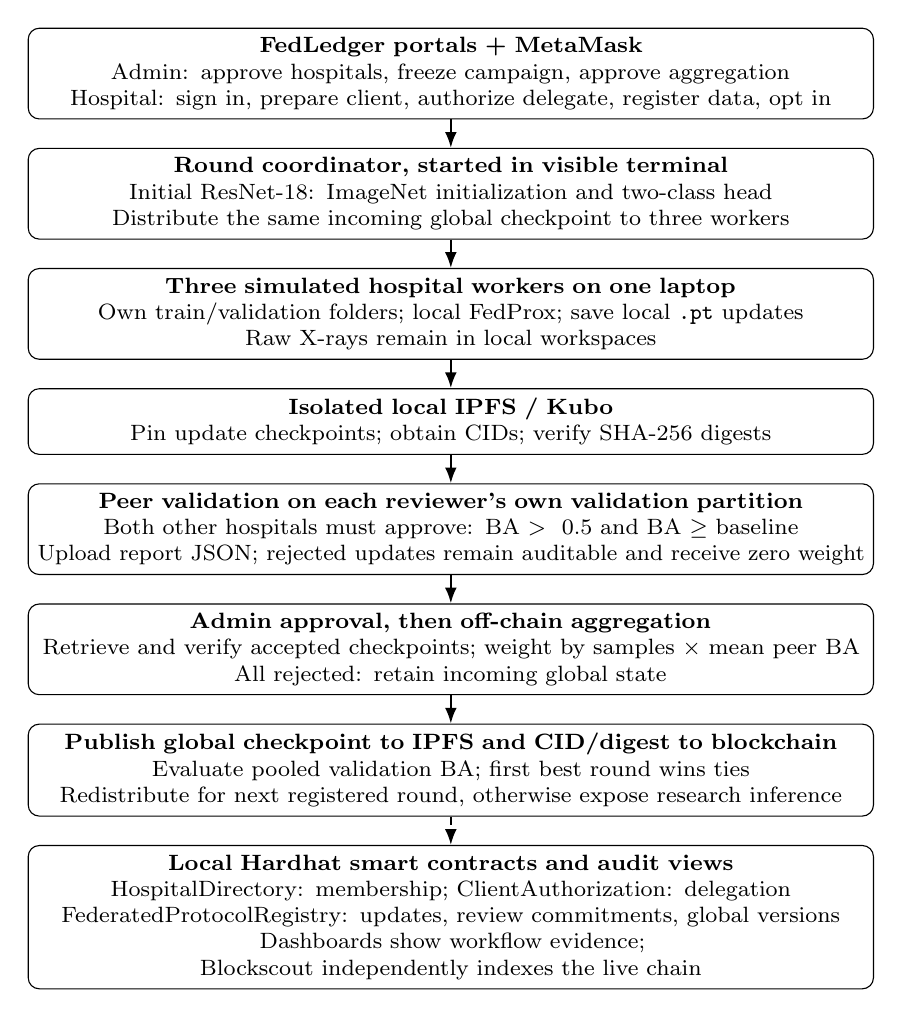
\begin{tikzpicture}[
  box/.style={draw,rounded corners,align=center,text width=10.5cm,
              minimum height=0.8cm,font=\footnotesize},
  arr/.style={-{Latex[length=2mm]},thick},
  node distance=0.36cm
]
\node[box] (portal) {\textbf{FedLedger portals + MetaMask}\\
Admin: approve hospitals, freeze campaign, approve aggregation\\
Hospital: sign in, prepare client, authorize delegate, register data, opt in};
\node[box,below=of portal] (coordinator) {\textbf{Round coordinator, started in visible terminal}\\
Initial ResNet-18: ImageNet initialization and two-class head\\
Distribute the same incoming global checkpoint to three workers};
\node[box,below=of coordinator] (hospitals) {\textbf{Three simulated hospital workers on one laptop}\\
Own train/validation folders; local FedProx; save local \texttt{.pt} updates\\
Raw X-rays remain in local workspaces};
\node[box,below=of hospitals] (storage) {\textbf{Isolated local IPFS / Kubo}\\
Pin update checkpoints; obtain CIDs; verify SHA-256 digests};
\node[box,below=of storage] (review) {\textbf{Peer validation on each reviewer's own validation partition}\\
Both other hospitals must approve: BA $>0.5$ and BA $\geq$ baseline\\
Upload report JSON; rejected updates remain auditable and receive zero weight};
\node[box,below=of review] (aggregate) {\textbf{Admin approval, then off-chain aggregation}\\
Retrieve and verify accepted checkpoints; weight by samples $\times$ mean peer BA\\
All rejected: retain incoming global state};
\node[box,below=of aggregate] (global) {\textbf{Publish global checkpoint to IPFS and CID/digest to blockchain}\\
Evaluate pooled validation BA; first best round wins ties\\
Redistribute for next registered round, otherwise expose research inference};
\node[box,below=of global] (chain) {\textbf{Local Hardhat smart contracts and audit views}\\
HospitalDirectory: membership; ClientAuthorization: delegation\\
FederatedProtocolRegistry: updates, review commitments, global versions\\
Dashboards show workflow evidence; Blockscout independently indexes the live chain};
\foreach \a/\b in {portal/coordinator,coordinator/hospitals,hospitals/storage,
storage/review,review/aggregate,aggregate/global}
  \draw[arr] (\a.south) -- (\b.north);
\draw[arr,dashed] (global.south) -- (chain.north);
\end{tikzpicture}
\doublespacing
\caption{System architecture of the FedLedger local research prototype. Raw source images remain in hospital data folders; checkpoints and reports are stored off-chain, while the development blockchain records workflow references and commitments.}
\label{fig:architecture}
\end{figure}

\section{Requirements Analysis}
\subsection{Functional Requirements}
\begin{enumerate}
    \item Support wallet-challenge hospital sign-in and administrator-token authentication.
    \item Support pending, approved, rejected, and suspended hospital states with applicable transitions and on-chain directory checks.
    \item Register local train/validation folders, class counts, file hashes, and patient mappings without uploading raw images.
    \item Register a campaign with exactly three approved participants, fixed parameters, data versions, and a declared round count; require participant opt-in.
    \item Train a local model, produce a checkpoint, and record its content reference and digest.
    \item Collect peer validation reports, decide update acceptance using the registered rule, and allow aggregation only after the workflow approval gate.
    \item Publish a new global checkpoint or retain the previous checkpoint when every update is rejected.
    \item Display progress, metrics, CIDs, transaction receipts, audit history, and permitted model-version predictions.
\end{enumerate}

\subsection{Non-functional Requirements}
The prototype aims for role-scoped access, integrity checks for registered inputs and downloaded artifacts, immutable campaign configuration, traceable workflow events, and recoverable pauses/retries at safe workflow boundaries. Its privacy goal is limited: raw images are not uploaded by the described workflow, but model updates may reveal information. It provides no formal differential-privacy or secure-aggregation guarantee. Its blockchain and IPFS services are local development infrastructure and do not establish production availability, performance, or independent institutional trust.

\section{Hardware and Software Specifications}
The user-reported development laptop runs Windows and has a Ryzen 7 250 processor, an NVIDIA RTX 5060 GPU with 8 GB VRAM, and 24 GB RAM. These are operator-provided specifications, not a hardware profile independently captured for every historical run. CUDA-enabled PyTorch is used for local training when available; final reproducibility reporting should record the actual driver and package versions. The documented implementation components are listed in Table~\ref{tab:software}.

\begin{table}[htbp]
\centering
\caption{Documented implementation components}
\label{tab:software}
\begin{tabularx}{\textwidth}{p{0.29\textwidth}Y}
\toprule
\textbf{Component} & \textbf{Role in the prototype} \\
\midrule
Python, PyTorch, ResNet-18 & Local image classification and model training/evaluation. \\
FedProx & Local objective regularization toward the incoming global parameters. \\
HTML, CSS, JavaScript & Separate administrator and hospital web interfaces; not a Streamlit application. \\
Python HTTP server and SQLite & Authenticated application APIs and workflow coordination state. \\
IPFS / Kubo & Local content-addressed storage for checkpoints and reports. \\
Hardhat 3 and Solidity & Local Ethereum-compatible development chain (chain ID 31337) and authorization/protocol contracts. \\
MetaMask & Hospital wallet login and signed local-client delegation. \\
Blockscout and Docker & Independent local chain explorer; separate from dashboard receipt views. \\
Rich & Terminal progress display during training. \\
\bottomrule
\end{tabularx}
\end{table}

\section{System Architecture}
The system separates local learning, coordination, artifact storage, ledger commitments, and portal operations. Hospital workers own local image access and local optimization. The coordinator owns campaign sequencing, policy evaluation, and aggregation. IPFS stores larger artifact bytes outside the ledger, while the chain stores compact references and workflow commitments. The portal and SQLite database provide operational views and coordination records. A content identifier locates stored bytes; a SHA-256 digest can detect a mismatch between expected and retrieved bytes; a transaction hash identifies a chain transaction. None of these checks proves correct labels, honest review, or clinical usefulness.

\subsection{Identity, Enrollment, and Data Setup}
A hospital signs a one-use login challenge with its wallet. The server verifies the signature and creates a temporary session. Administrator approval updates the hospital directory; an approved owner separately delegates a local training-client key through a signed authorization message. This proves control of a wallet or delegated key, not the applicant's real-world identity. Readiness heartbeats are self-reported and expire.

Each hospital's data folder contains train and validation subfolders for NORMAL and PNEUMONIA, with an optional \texttt{patients.csv} mapping relative paths to patient IDs. Registration checks hashes, folder boundaries, both-class coverage, and patient overlap where IDs are available. Different patient-ID namespaces do not prove that the underlying people differ, and byte-level duplicate checks do not rule out all transformed copies.

\subsection{Local Training Objective}
The initial global model is an ImageNet-initialized ResNet-18 with its final layer replaced by a two-class head \cite{he2016resnet}. Portal campaigns retrieve the preserved initial checkpoint, rather than starting from the previously selected pneumonia checkpoint. Images are converted to RGB and resized to $224\times224$. Training uses random rotation up to $10^{\circ}$ and brightness/contrast jitter of 0.1; evaluation omits these random augmentations. Both use ImageNet normalization. The local optimizer is Adam with learning rate $10^{-4}$, batch size 32, class-weighted cross-entropy and a FedProx penalty \cite{li2020fedprox}. For hospital $k$, local parameters $w$ are optimized against incoming global parameters $w_t$ using
\begin{equation}
    \mathcal{L}_{k}(w) = \mathcal{L}_{\mathrm{CE},k}(w) + \frac{\mu}{2}\lVert w-w_t\rVert_2^2,
\end{equation}
where the registered configuration uses $\mu=0.01$. The proximal term discourages local parameters from moving too far from the current global model. It does not itself validate a client's update or protect the update from inference.

\subsection{Peer Acceptance and Aggregation}
Each update is reviewed by the other two participants. On a reviewer's validation partition, a candidate must have balanced accuracy strictly greater than 0.5 and at least as high as the incoming global model. Both peers must approve. Missing, duplicate, or invalid reviews reject an update; model loading also checks tensor structure and finite values. Balanced accuracy is
\begin{equation}
    \mathrm{BA}=\frac{1}{2}\left(\frac{TP}{TP+FN}+\frac{TN}{TN+FP}\right).
\end{equation}
For accepted update $i$, the project uses
\begin{equation}
    m_i=n_i\,\bar{b}_i,\qquad
    \alpha_i=\frac{m_i}{\sum_{j\in\mathcal{A}}m_j},\qquad
    w_{t+1}=\sum_{i\in\mathcal{A}}\alpha_i w_i,
\end{equation}
where $n_i$ is the local training sample count, $\bar{b}_i$ is its mean peer balanced accuracy, and $\mathcal{A}$ is the set of accepted updates. Rejected updates receive zero weight. Floating-point state tensors use the weighted average; integer buffers use the existing weighted-average-then-round convention. If $\mathcal{A}$ is empty, the incoming global model is retained. The weights are derived from validation scores, so these validation sets participate in model development rather than serving as independent final tests. Administrator approval releases aggregation execution but cannot override the registered acceptance rule or select updates by hand.

\section{System Diagrams}
\subsection{Use-case View}
Figure~\ref{fig:usecase} shows the primary responsibilities of the administrator and hospital participant. The diagram describes the software workflow and does not imply that a hospital is a real external institution.

\begin{figure}[htbp]
\centering
\singlespacing
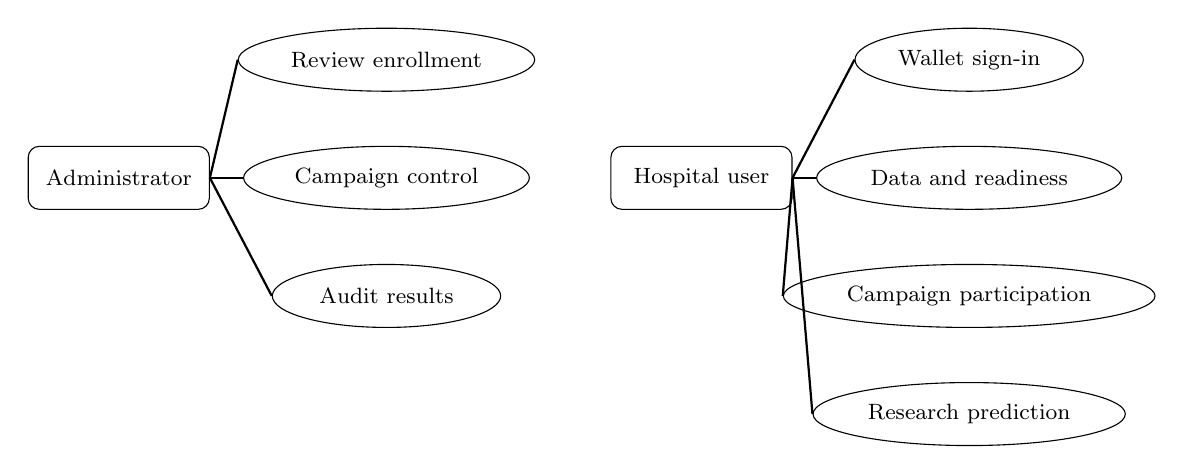
\begin{tikzpicture}[
  actor/.style={draw,rounded corners,minimum width=2.3cm,minimum height=0.8cm,align=center,font=\footnotesize},
  usecase/.style={draw,ellipse,minimum width=2.9cm,minimum height=0.8cm,align=center,font=\footnotesize},
  arr/.style={thick}
]
\node[actor] (admin) at (0,1.2) {Administrator};
\node[actor] (hospital) at (7.4,1.2) {Hospital user};
\node[usecase] (review) at (3.4,2.7) {Review enrollment};
\node[usecase] (campaign) at (3.4,1.2) {Campaign control};
\node[usecase] (audit) at (3.4,-0.3) {Audit results};
\node[usecase] (auth) at (10.8,2.7) {Wallet sign-in};
\node[usecase] (data) at (10.8,1.2) {Data and readiness};
\node[usecase] (participate) at (10.8,-0.3) {Campaign participation};
\node[usecase] (predict) at (10.8,-1.8) {Research prediction};
\draw[arr] (admin.east) -- (review.west);
\draw[arr] (admin.east) -- (campaign.west);
\draw[arr] (admin.east) -- (audit.west);
\draw[arr] (hospital.east) -- (auth.west);
\draw[arr] (hospital.east) -- (data.west);
\draw[arr] (hospital.east) -- (participate.west);
\draw[arr] (hospital.east) -- (predict.west);
\end{tikzpicture}
\doublespacing
\caption{Use-case view of role-specific prototype functions.}
\label{fig:usecase}
\end{figure}

\subsection{Round Workflow}
The principal exchange is shown in Figure~\ref{fig:workflow}. Model parameters move from the global checkpoint to each hospital; local images do not follow that path. Updates and reports are persisted as off-chain artifacts, while identifiers and commitments are recorded on the development chain.

\begin{figure}[htbp]
\centering
\singlespacing
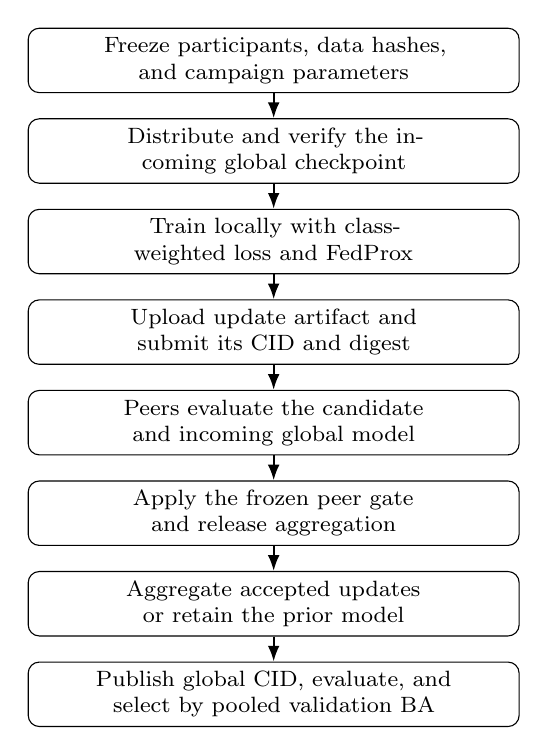
\begin{tikzpicture}[
  workflowbox/.style={draw,rounded corners,align=center,text width=6.0cm,minimum height=0.72cm,font=\footnotesize},
  arr/.style={-{Latex[length=2mm]},thick}
]
\node[workflowbox] (s1) at (0,0) {Freeze participants, data hashes, and campaign parameters};
\node[workflowbox] (s2) at (0,-1.15) {Distribute and verify the incoming global checkpoint};
\node[workflowbox] (s3) at (0,-2.30) {Train locally with class-weighted loss and FedProx};
\node[workflowbox] (s4) at (0,-3.45) {Upload update artifact and submit its CID and digest};
\node[workflowbox] (s5) at (0,-4.60) {Peers evaluate the candidate and incoming global model};
\node[workflowbox] (s6) at (0,-5.75) {Apply the frozen peer gate and release aggregation};
\node[workflowbox] (s7) at (0,-6.90) {Aggregate accepted updates or retain the prior model};
\node[workflowbox] (s8) at (0,-8.05) {Publish global CID, evaluate, and select by pooled validation BA};
\draw[arr] (s1.south) -- (s2.north);
\draw[arr] (s2.south) -- (s3.north);
\draw[arr] (s3.south) -- (s4.north);
\draw[arr] (s4.south) -- (s5.north);
\draw[arr] (s5.south) -- (s6.north);
\draw[arr] (s6.south) -- (s7.north);
\draw[arr] (s7.south) -- (s8.north);
\end{tikzpicture}
\doublespacing
\caption{Federated round workflow as implemented in the project handoff.}
\label{fig:workflow}
\end{figure}

\subsection{Conceptual Data Model}
Figure~\ref{fig:erd} presents the main entities. It is a conceptual model: specific SQLite columns and on-chain structures differ by component, and the drawing does not imply that the full model or image data are stored on-chain.

\begin{figure}[htbp]
\centering
\singlespacing
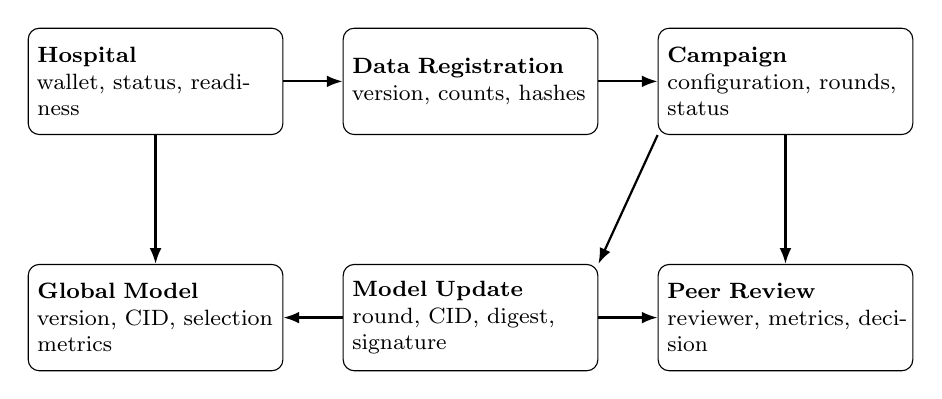
\begin{tikzpicture}[
  ent/.style={draw,rounded corners,align=left,text width=3.0cm,minimum height=1.35cm,font=\footnotesize},
  rel/.style={-{Latex[length=2mm]},thick}
]
\node[ent] (hospital) at (0,2) {\textbf{Hospital}\\wallet, status, readiness};
\node[ent] (dataset) at (4.0,2) {\textbf{Data Registration}\\version, counts, hashes};
\node[ent] (campaign) at (8.0,2) {\textbf{Campaign}\\configuration, rounds, status};
\node[ent] (update) at (4.0,-1) {\textbf{Model Update}\\round, CID, digest, signature};
\node[ent] (review) at (8.0,-1) {\textbf{Peer Review}\\reviewer, metrics, decision};
\node[ent] (global) at (0,-1) {\textbf{Global Model}\\version, CID, selection metrics};
\draw[rel] (hospital.east) -- (dataset.west);
\draw[rel] (dataset.east) -- (campaign.west);
\draw[rel] (campaign.south) -- (review.north);
\draw[rel] (campaign.south west) -- (update.north east);
\draw[rel] (update.east) -- (review.west);
\draw[rel] (hospital.south) -- (global.north);
\draw[rel] (update.west) -- (global.east);
\end{tikzpicture}
\doublespacing
\caption{Conceptual entities and relationships in the campaign and audit workflow.}
\label{fig:erd}
\end{figure}

% Chapter 4
\chapter{System Implementation}
\section{Implementation Overview}
The implementation is organized into a browser-based application, local hospital workers, a coordinator, an artifact-storage adapter, and blockchain protocol wrappers. The Python HTTP server exposes authenticated APIs and serves separate administrator and hospital interfaces built with HTML, CSS, and JavaScript. SQLite stores application, session, readiness, campaign, participation, and coordination state. The training workers and coordinator run as separate processes; the dashboard's campaign start control returns a command for execution in a visible terminal rather than launching hidden training.

\section{Enrollment and Authorization}
Hospital enrollment begins in a pending state and is reviewed by an administrator. Approved hospitals prepare a local training client and sign a delegation message; the server checks the signature before recording eligibility through the client-authorization contract. The owner wallet's private key is not exported by the portal; the delegated development client has a locally stored signing key. Rejected applications do not have a direct status transition in the current interface, and approval status must agree with the local directory and live contract membership. Because the active development chain can be replaced, prior approvals and receipts require careful interpretation after a reset.

\section{Data Registration and Campaign Setup}
Data registration is local to a hospital workspace. The registration process checks data folder boundaries, image hashes, patient mapping overlap, class availability, and relevant metadata. The browser-facing responses expose the owning hospital's setup and aggregate coordination information according to role. However, the local Python service scans image files, writes manifests containing absolute paths, hashes and patient mappings, and stores manifest references centrally on this laptop. The coordinator reads these manifests and dispatches local worker jobs. Raw image bytes are not uploaded to IPFS or blockchain, but the single-machine operator can access all hospital folders; the prototype does not yet provide remote institutional data isolation. A campaign freezes participants, data versions, source hashes, hyperparameters, and round count. All selected hospitals opt in before the coordinator proceeds. A process-level training lock prevents overlapping training executions on this local system; it is not a distributed multi-server locking protocol.

\section{Training and Round Coordination}
For each round, workers load the incoming global checkpoint after verifying its digest, train locally, and serialize their model state. They upload the checkpoint to IPFS and submit the CID, digest, and round through their delegated signer. The other participating hospitals evaluate the update against their own validation partitions and compare it with the incoming model. The coordinator collects those results and applies the fixed peer gate. Following an aggregation-release action, accepted states are combined off-chain; rejected submissions receive no weight. The new global checkpoint is published and referenced on-chain, then evaluated by the participants.

\section{Artifact Integrity and Audit}
IPFS holds checkpoint and validation-report bytes, while the blockchain stores authorization state, model references, and validation commitments. The application hashes serialized artifacts so a retrieved file can be checked against its expected digest. SQLite stores application and coordination state needed by the portals. Specifically, \texttt{HospitalDirectory} tracks membership, \texttt{ClientAuthorization} tracks delegated consent, and \texttt{FederatedProtocolRegistry} tracks protocol records. Update/global CIDs and digests are committed on-chain. Peer-review transactions commit report evidence hashes and decision data; peer-report CIDs are retained in off-chain artifacts rather than directly in those review transactions. Rejected checkpoints are not deleted from IPFS merely because their aggregation weight is zero. Audit history supports inspection of model versions, peer decisions, aggregation evidence, transaction references, and workflow status. These mechanisms improve traceability and detect byte-level mismatch but do not prove semantic correctness or prevent all forms of model inversion and data inference.

\section{Prediction Interface}
The research prediction interface loads a selected, hash-checked checkpoint and applies the evaluation preprocessing before running ResNet-18. It reports NORMAL/PNEUMONIA scores. The scores are uncalibrated model outputs, not validated diagnostic probabilities, and the interface does not reliably establish that each uploaded image is a chest radiograph. Uploaded prediction images are handled in memory and are not written to the blockchain.

\section{Security and Operational Limitations}
The prototype's trust boundary is local. Application roles limit API access, but an operator with access to the laptop can access local files. The described workflow does not implement differential privacy or secure aggregation, and exchanged model weights can reveal training information. Wallet signatures establish key control only. The local Hardhat chain and isolated IPFS node are development services rather than a resilient multi-institution deployment. A real deployment would require institutional identity verification, remote hospital agents and authenticated transport, secret and network isolation, persistent infrastructure, privacy/security review, and governance agreements. Hardhat development state is normally ephemeral when its node is stopped; a replacement chain cannot be represented as the original chain. Saved receipts remain historical evidence, and live verification requires the matching chain instance. Blockscout indexes that live development chain independently but does not make it persistent or clinically trustworthy.

% Chapter 5
\chapter{Preliminary Results}
\section{Evaluation Protocol and Evidence Boundaries}
The evidence distinguishes an earlier architecture experiment from later dashboard-driven campaigns. The cases below are identified by run or campaign ID and are not an exhaustive claim that only two runs exist. The values below are validation results saved with those respective runs, not independent test-set estimates. The selected checkpoint is chosen using pooled validation balanced accuracy; ties retain the earlier selected round. Test data do not select rounds or parameters. No corrected-v2 performance is available, and no current FedAvg comparison is established.

\section{Earlier Architecture Experiment}
Run \texttt{run\_20261020T093433\_860908Z} used ResNet-18, FedProx $\mu=0.01$, seed 42, three local epochs, and twenty rounds. Round 11 was selected using validation balanced accuracy. Table~\ref{tab:architecture-run} gives the recorded selected validation metrics. Peer gating rejected many later updates, and some later rounds retained the previous model; this retention must not be described as continued learning or convergence.

\begin{table}[htbp]
\centering
\caption{Selected validation metrics from the earlier architecture experiment}
\label{tab:architecture-run}
\begin{tabular}{lr}
\toprule
\textbf{Measure} & \textbf{Recorded value} \\
\midrule
Selected round & 11 of 20 \\
Validation accuracy & 98.7005\% \\
Validation balanced accuracy & 98.7005\% \\
Validation ROC-AUC & 0.998578 \\
\bottomrule
\end{tabular}
\end{table}

\section{Dashboard Smoke Campaign}
Campaign \url{34c72e51-c98a-4a99-be9a-a540dce32a35} involved SNRSE, ASTER, and RGRI for one round with three local epochs, seed 42, and $\mu=0.01$. All three updates were accepted after both peer reviewers approved. The round took 404.85 seconds according to the saved record. A saved verification script checked the mechanical consistency of peer decisions, aggregation weights, tensors, checkpoint hash, and then-live transaction receipts. This is a project-local consistency check, not an external audit or independent clinical validation.

\begin{table}[htbp]
\centering
\caption{Recorded pooled validation metrics for the dashboard smoke campaign}
\label{tab:smoke-results}
\begin{tabular}{lr}
\toprule
\textbf{Measure} & \textbf{Recorded value} \\
\midrule
Validation images & 1,354 \\
Accuracy & 98.3013\% \\
Balanced accuracy & 98.3020\% \\
Sensitivity & 98.5185\% \\
Specificity & 98.0854\% \\
Precision & 98.0826\% \\
F1 score & 0.983001 \\
ROC-AUC & 0.998970 \\
Round duration & 404.85 seconds \\
\bottomrule
\end{tabular}
\end{table}

The recorded confusion counts are TP=665, FN=10, FP=13, and TN=666, as shown in Table~\ref{tab:confusion}. These counts produce the reported sensitivity and specificity on the smoke validation set.

\begin{table}[htbp]
\centering
\caption{Recorded confusion counts for the dashboard smoke campaign}
\label{tab:confusion}
\begin{tabular}{lrr}
\toprule
 & \textbf{Predicted PNEUMONIA} & \textbf{Predicted NORMAL} \\
\midrule
Actual PNEUMONIA & 665 (TP) & 10 (FN) \\
Actual NORMAL & 13 (FP) & 666 (TN) \\
\bottomrule
\end{tabular}
\end{table}

\section{Later Completed Portal Campaign}
The preserved record for campaign \url{dbcb01f4-e574-4027-8f54-d9772d08c8d2}
also reports a completed one-round campaign with seed 42, three local epochs,
and $\mu=0.01$. It used registered code-based hospital workspaces and accepted
all three updates. It is a distinct workflow execution, not an additional seed
or an independent external test. Its saved pooled validation values are:
\begin{table}[htbp]
\centering
\caption{Saved validation results for the later one-round portal campaign}
\begin{tabular}{lr}
\toprule
\textbf{Measure} & \textbf{Recorded value} \\
\midrule
Accuracy & 98.6706\% \\
Balanced accuracy & 98.6693\% \\
F1 score & 0.986607 \\
ROC-AUC & 0.998859 \\
Round duration & 481.17 seconds \\
\bottomrule
\end{tabular}
\end{table}
No reviewed-v2 migration or external independence is established by these
metric files. Higher validation accuracy in this later campaign must not be
interpreted as a controlled improvement, a corrected-data result, or evidence
that the earlier leakage concern has been resolved.

\section{Data Leakage Review and Interpretation}
A later transformed-image review of campaign \texttt{34c72e51} found a probable related radiograph pair crossing its training/validation boundary. This means that its validation score may be optimistic and is retained only as preliminary smoke-test evidence. It must not be transferred to the corrected data version or represented as independent final accuracy. The reviewed v2 copy groups the suspected image family in training and changes the staging counts slightly, but no completed evaluation of that reviewed version is established by the inspected evidence. Perceptual screening can also miss additional transformations, and inferred patient IDs do not certify patient independence.

The completed experiments demonstrate that the workflow can execute local training, peer review, gated aggregation, artifact storage, and ledger recording under the recorded local setup. They do not prove clinical validity, privacy against model-inference attacks, Byzantine robustness, or generalization to independent hospitals. Software and synthetic workflow checks test system behavior, not model accuracy.

\section{Data Preparation Snapshot}
Table~\ref{tab:v2-counts} records the corrected staging counts supplied in the handoff. These are image counts, not unique-patient counts. The staging names \texttt{hospital1}--\texttt{hospital3} are folder labels, not permanent dashboard hospital identities; the actual campaign mapping must be read from its frozen registration and manifests. They describe an unevaluated staging copy and must not be confused with the original smoke-campaign partitions.

\begin{table}[htbp]
\centering
\caption{Corrected staging v2 image counts by hospital and split}
\label{tab:v2-counts}
\resizebox{\textwidth}{!}{\begin{tabular}{lrrrr}
\toprule
\textbf{Hospital folder} & \textbf{Train NORMAL} & \textbf{Train PNEUMONIA} & \textbf{Val NORMAL} & \textbf{Val PNEUMONIA} \\
\midrule
hospital1 & 1,899 & 814 & 473 & 203 \\
hospital2 & 570 & 1,058 & 142 & 264 \\
hospital3 & 251 & 834 & 63 & 208 \\
\bottomrule
\end{tabular}}
\end{table}

\section{Local Evidence Sources and Reproducibility}
The numerical tables were checked against preserved files under
\texttt{multiseed\_outputs/}; they are rounded for presentation, not new
measurements. The principal sources are:
\begin{itemize}
\item \path{multiseed_outputs/architecture/run_20261020T093433_860908Z/validation_metrics.json},
\path{selection.json}, and \path{results_review.json} in that run folder.
\item \path{multiseed_outputs/portal_campaigns/34c72e51-c98a-4a99-be9a-a540dce32a35/history.json}
and \path{result_verification.json} in that campaign folder.
\item \path{multiseed_outputs/portal_campaigns/dbcb01f4-e574-4027-8f54-d9772d08c8d2/history.json},
\path{status.json}, \path{registration.json}, and \path{selection.json} in that folder.
\item \path{multiseed_outputs/hospital_reviewed_v2_latest.json} and
\path{multiseed_outputs/campaign_leakage_review/20261022T080906_451339Z/REPORT.md}.
\end{itemize}
The different runs have different registered data references. Their scores
must not be pooled as repeated seeds or compared as if only the algorithm
changed. No matched FedAvg comparison, patient-cluster confidence interval,
or statistically supported algorithm ranking is established. The original
dataset and historical artifacts were not modified during this report review.

% Chapter 6
\chapter{Project Schedule}
\section{Status and Planned Work}
The project context documents a completed prototype and historical smoke experiment, but no later corrected-data evaluation. Table~\ref{tab:schedule} distinguishes completed work from the next research tasks. The durations in Figure~\ref{fig:gantt} are indicative planning estimates only; they are not dates or completed work records.

\begin{table}[htbp]
\centering
\caption{Project schedule and current status}
\label{tab:schedule}
\begin{tabularx}{\textwidth}{p{0.36\textwidth}p{0.20\textwidth}Y}
\toprule
\textbf{Activity} & \textbf{Status} & \textbf{Output / next action} \\
\midrule
Literature review and scope definition & Draft prepared & Ten related studies plus foundational method papers cited; departmental review remains required. \\
Prototype architecture and portal workflow & Implemented & Authentication, registration, dashboards, coordinator, IPFS, and local-chain workflow. \\
Initial architecture and smoke experiments & Completed & Preserve both runs as distinct historical evidence. \\
Check approvals and client delegation & Conditional & After chain replacement, reapprove and reauthorize affected clients; inspect live state before declaring this pending. \\
Register corrected v2 data & Pending & Register the reviewed copy as a new immutable data version. \\
Longer pre-registered experiment and repeated seeds & Planned & Freeze configuration and stopping plan; add seed support explicitly if needed. \\
Independent patient-wise evaluation & Planned & Obtain and audit a genuinely independent test cohort. \\
\bottomrule
\end{tabularx}
\end{table}

\begin{figure}[htbp]
\centering
\singlespacing
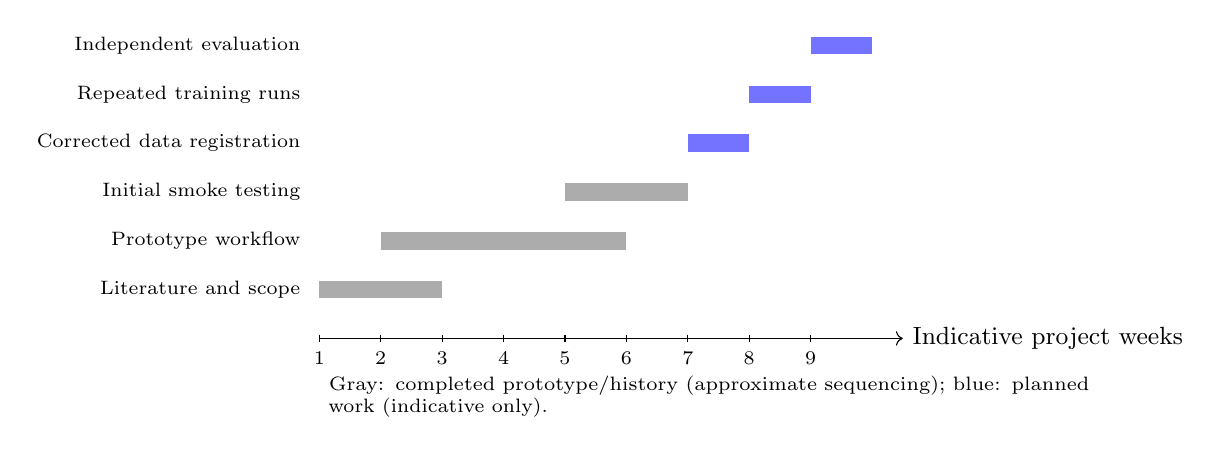
\begin{tikzpicture}[x=0.78cm,y=0.62cm]
\draw[->] (0,0) -- (9.5,0) node[right,font=\small]{Indicative project weeks};
\foreach \x [count=\week from 1] in {0,...,8} {\draw (\x,0.08) -- (\x,-0.08) node[below,font=\scriptsize]{\week};}
\foreach \y/\taskname/\start/\finish/\barcolor in {
  1/Literature and scope/0/2/gray!65,
  2/Prototype workflow/1/5/gray!65,
  3/Initial smoke testing/4/6/gray!65,
  4/Corrected data registration/6/7/blue!55,
  5/Repeated training runs/7/8/blue!55,
  6/Independent evaluation/8/9/blue!55
} {
  \node[anchor=east,font=\scriptsize] at (-0.15,\y) {\taskname};
  \fill[\barcolor] (\start,\y-0.18) rectangle (\finish,\y+0.18);
}
\node[font=\scriptsize,anchor=west,text width=10cm,align=left] at (0,-1.2) {Gray: completed prototype/history (approximate sequencing); blue: planned work (indicative only).};
\end{tikzpicture}
\doublespacing
\caption{Indicative schedule. Bars are a proposed planning sequence, not a dated project log.}
\label{fig:gantt}
\end{figure}

% Chapter 7
\chapter{Conclusion}
FedLedger implements a coordinator-based federated-learning research prototype for two-class pneumonia classification. Its workflow combines local ResNet-18 training with FedProx, peer validation, a project-defined update gate and aggregation rule, IPFS artifact storage, local blockchain commitments, and role-specific portals. The supplied experiment history records that the workflow completed both an earlier multi-round architecture experiment and a one-round dashboard smoke campaign.

The available numerical metrics are validation results, not independent test estimates. In particular, a probable transformed-image family crossing the smoke campaign's training/validation split makes that campaign unsuitable as final accuracy evidence. The corrected v2 data are unevaluated. The prototype therefore demonstrates workflow integration and audit mechanics under local conditions, but does not establish clinical performance, privacy guarantees against model leakage, Byzantine robustness, or deployment readiness.

The next steps are to check live approvals and delegated-client authorization after any chain replacement, register and audit the reviewed data as a new immutable version where needed, pre-register a longer experiment with repeated seeds, and evaluate a frozen model on a genuinely independent patient-wise test cohort. Future comparisons should include a matched baseline such as FedAvg, uncertainty estimates, explicit data provenance, and a documented assessment of privacy, security, and operational costs.

\singlespacing
\begin{thebibliography}{99}
\addcontentsline{toc}{chapter}{Bibliography}
\bibitem{wang2026bcfl}
X. Wang et al., ``Securing Federated Learning With Blockchain in the Medical
Field: Systematic Literature Review,'' \textit{Journal of Medical Internet
Research}, vol. 28, e79052, 2026. \url{https://doi.org/10.2196/79052}.

\bibitem{zhu2023blockfed}
J. Zhu, J. Cao, D. Saxena, S. Jiang, and H. Ferradi,
``Blockchain-Empowered Federated Learning: Challenges, Solutions, and Future
Directions,'' \textit{ACM Computing Surveys}, vol. 55, no. 11, article 240,
2023. \url{https://doi.org/10.1145/3570953}.

\bibitem{shayan2021biscotti}
M. Shayan, C. Fung, C. J. M. Yoon, and I. Beschastnikh,
``Biscotti: A Blockchain System for Private and Secure Federated Learning,''
\textit{IEEE Transactions on Parallel and Distributed Systems}, vol. 32,
no. 7, pp. 1513--1525, 2021.
\url{https://doi.org/10.1109/TPDS.2020.3044223}.

\bibitem{li2021bflc}
Y. Li, C. Chen, N. Liu, H. Huang, Z. Zheng, and Q. Yan,
``A Blockchain-Based Decentralized Federated Learning Framework with Committee
Consensus,'' \textit{IEEE Network}, vol. 35, no. 1, pp. 234--241, 2021.
\url{https://doi.org/10.1109/MNET.011.2000263}.

\bibitem{ferretti2025resilient}
S. Ferretti, L. Cassano, G. Cialone, J. D'Abramo, and F. Imboccioli,
``Decentralized coordination for resilient federated learning: A blockchain-based
approach with smart contracts and decentralized storage,''
\textit{Computer Communications}, article 108112, 2025.
\url{https://doi.org/10.1016/j.comcom.2025.108112}.

\bibitem{miao2022pbfl}
Y. Miao, Z. Liu, H. Li, K. K. R. Choo, and R. H. Deng,
``Privacy-Preserving Byzantine-Robust Federated Learning via Blockchain Systems,''
\textit{IEEE Transactions on Information Forensics and Security}, vol. 17,
pp. 2848--2861, 2022. \url{https://doi.org/10.1109/TIFS.2022.3196274}.

\bibitem{subramanian2022healthcare}
M. Subramanian, V. Rajasekar, Sathishkumar V. E., K. Shanmugavadivel,
and P. S. Nandhini, ``Effectiveness of Decentralized Federated Learning
Algorithms in Healthcare: A Case Study on Cancer Classification,''
\textit{Electronics}, vol. 11, no. 24, article 4117, 2022.
\url{https://doi.org/10.3390/electronics11244117}.

\bibitem{peng2023covid}
L. Peng et al., ``Evaluation of federated learning variations for COVID-19
diagnosis using chest radiographs from 42 US and European hospitals,''
\textit{Journal of the American Medical Informatics Association}, vol. 30,
no. 1, pp. 54--63, 2023 (published online 2022).
\url{https://doi.org/10.1093/jamia/ocac188}.

\bibitem{darzi2024covid}
E. Darzi, N. M. Sijtsema, and P. M. A. van Ooijen,
``A comparative study of federated learning methods for COVID-19 detection,''
\textit{Scientific Reports}, vol. 14, article 3944, 2024.
\url{https://doi.org/10.1038/s41598-024-54323-2}.

\bibitem{rashidi2024detection}
G. Rashidi, D. Bounias, M. Bujotzek, A. Mart\'{i}nez Mora, P. Neher,
and K. H. Maier-Hein, ``The potential of federated learning for self-configuring
medical object detection in heterogeneous data distributions,''
\textit{Scientific Reports}, vol. 14, article 23844, 2024.
\url{https://doi.org/10.1038/s41598-024-74577-0}.

\bibitem{li2020fedprox}
T. Li, A. K. Sahu, M. Zaheer, M. Sanjabi, A. Talwalkar, and V. Smith,
``Federated Optimization in Heterogeneous Networks,''
\textit{Proceedings of Machine Learning and Systems}, vol. 2,
pp. 429--450, 2020. \url{https://arxiv.org/abs/1812.06127}.

\bibitem{he2016resnet}
K. He, X. Zhang, S. Ren, and J. Sun,
``Deep Residual Learning for Image Recognition,''
\textit{Proceedings of the IEEE Conference on Computer Vision and Pattern
Recognition}, pp. 770--778, 2016.
\url{https://openaccess.thecvf.com/content_cvpr_2016/html/He_Deep_Residual_Learning_CVPR_2016_paper.html}.
\end{thebibliography}

% Appendices
\appendix
\chapter{Turnitin Similarity Report}
The verified similarity report was not included among the supplied project files. Insert the institution-generated report here after the final manuscript is checked. The similarity percentage on the declaration page must match the verified result; it must not be estimated.

\chapter{Supplied Base Papers}
The two designated base references used to frame the literature review are:
\begin{enumerate}
    \item X. Wang et al., ``Securing Federated Learning With Blockchain in the Medical Field: Systematic Literature Review,'' \textit{Journal of Medical Internet Research}, vol. 28, e79052, 2026 \cite{wang2026bcfl}.
    \item J. Zhu et al., ``Blockchain-Empowered Federated Learning: Challenges, Solutions, and Future Directions,'' \textit{ACM Computing Surveys}, vol. 55, no. 11, article 240, 2023 \cite{zhu2023blockfed}.
\end{enumerate}
Publisher or author links are provided in the bibliography. This verification received the LaTeX draft rather than the base-paper PDFs. Attach authorized source PDFs separately only if required by the department.

\end{document}